\documentclass[11pt,german,hideothersubsections]{beamer}

\usepackage{hyperref}
\usepackage{amsmath,nicefrac,booktabs,mathabx}
\usepackage{natbib}
\usepackage{url}
\usepackage{textpos}
\usepackage{listings}
\definecolor{Rblau}{rgb}{.3,.6,.9}

\lstset{language=R,
        basicstyle=\ttfamily\footnotesize,
        keywordstyle=\color{blue}\bfseries,
        identifierstyle=\color{Rblau},
        commentstyle=\color{gray},
        stringstyle=\color{green}\ttfamily,
        showstringspaces=false,
        frame=tb}



\bibpunct{(}{)}{;}{a}{,}{,}
\usepackage[english]{babel}
\usepackage[latin1]{inputenc}
\usepackage{helvet}
\usepackage{graphicx}
\usepackage{color}
\usepackage{multirow,dcolumn}
\usepackage{ragged2e}
\usepackage{xcolor}
\usepackage{colortbl}
\usepackage{tikz}
\usetikzlibrary{calc}
\usepackage{booktabs}
\colorlet{tablesubheadcolor}{gray!25}
\colorlet{tableheadcolor}{gray!40}
\colorlet{tablerowcolor}{gray!15.0}
\usetheme[english]{Gesis}
\setbeamertemplate{navigation symbols}{}
\setbeamertemplate{footline}[frame number]%{\hspace*{.2cm}\insertframenumber}
\setbeamerfont{caption}{size=\footnotesize}
\usefonttheme[onlylarge]{structuresmallcapsserif} % alte Schrift

\newcommand{\R}[1]{{\tt \color{blue}  #1}}
\newtheorem{thm}{Theorem}
\newtheorem{rem}{Bemerkung}
\newtheorem{lem}{Lemma}

\definecolor{hellgrau}{rgb}   {0.109375,  0.40625,   0.51953125}
\definecolor{dunkelgrau}{rgb} {0.009375,  0.30625,   0.41953125}
\definecolor{dunkelgrau2}{rgb}{0.009375,  0.20625,   0.31953125}
\definecolor{hellbraun}{rgb}  {0.9140625, 0.8984375, 0.8046875}
\definecolor{hellbraun2}{rgb} {.95,       0.9,       0.8}
\definecolor{alertred}{rgb}   {0.8515625, 0.3828125, 0.08984375}
\definecolor{orange}{rgb}{1,0.5,0}


\setbeamercolor{firstsecslide}{fg=white,bg=dunkelgrau}
\setbeamertemplate{blocks}[rounded][shadow=true]

\newcolumntype{d}[0]{D{,}{.}{6}}

\newenvironment{itemizeol}{\begin{itemize}[<+->]}{\end{itemize}}
\newenvironment{descriptionol}{\begin{description}[<+->]}{\end{description}}

\newcolumntype{V}[1]{%
  >{\RaggedRight\hspace{0pt}}p{#1}%
}

\newcommand{\emphred}[1]{\textcolor{alertred}{#1}}
\newcommand{\emphcol}[1]{\textcolor{dunkelgrau}{\slshape #1}}

\setcounter{tocdepth}{1}
\setbeamercolor*{section in toc}{fg=hellgrau}
\setbeamertemplate{bibliography item}[default]

\makeatother
\addtobeamertemplate{frametitle}{}{%
\begin{textblock*}{100mm}(.91\textwidth,-1cm)

\includegraphics[height=1cm,width=2cm]{../../graphs/logos/GESIS_Logo_kompakt_en.jpg}
\end{textblock*}}




\title[Day 1]{Tutorial: Sampling, Weighting and Estimation\\ \Large{Day 2} }
%\subtitle{Umgang am Beispiel von Telefonstichproben}

\author[M. Sand]{Stefan Zins, Matthias Sand\\ and Jan-Philipp Kolb\\ \vspace{.5cm} \footnotesize{GESIS - Leibniz Institute\\ for the Social Sciences}}
%\institute{\includegraphics[width=4.5cm]{GESIS_Logo_informell}}
\date[]{\color{dunkelgrau}\footnotesize%
\begin{minipage}{8cm}%
\begin{center}%
\scriptsize{
\textbf{GESIS Summer School}\\ \tiny{Cologne, Germany}%
}\\
\vspace{0.25cm}
\textbf{August 25th, 2015}%

\end{center}%
\end{minipage}}%


\usepackage{Sweave}
\begin{document}
\Sconcordance{concordance:Day2.tex:Day2.Rnw:%
1 103 1 1 0 2 1 1 12 10 1 1 2 1 0 1 1 5 0 1 1 6 0 1 2 6 1 1 2 1 0 1 1 5 %
0 2 1 5 0 1 1 6 0 1 2 1 1 1 2 7 0 1 2 6 1 1 2 1 0 1 1 11 0 3 1 10 0 1 2 %
14 1 1 2 1 0 1 1 6 0 1 2 1 1 1 2 1 0 1 1 12 0 1 2 13 1 1 2 1 0 1 3 2 0 %
1 1 6 0 1 2 11 1 1 2 1 0 1 5 4 0 1 1 11 0 1 2 5 1 1 2 1 0 1 1 1 2 1 0 1 %
2 1 0 1 2 1 0 1 1 1 4 3 0 1 2 5 0 1 3 6 1 1 15 17 0 1 2 10 1 1 3 2 0 2 %
1 3 0 1 2 20 1 1 2 1 0 1 1 5 0 1 1 6 0 1 2 10 1 1 3 2 0 1 1 11 0 1 1 7 %
0 1 2 13 1 1 2 1 0 1 1 6 0 1 2 10 1 1 3 2 0 1 1 9 0 2 1 10 0 1 2 5 1 1 %
11 13 0 1 2 13 1 1 2 1 0 1 1 12 0 1 2 14 1 1 2 1 0 2 1 1 4 3 0 3 1 7 0 %
1 2 9 1 1 2 1 0 2 1 12 0 1 2 20 1 1 2 1 0 3 1 6 0 3 1 6 0 1 2 22 1 1 7 %
6 0 1 1 6 0 1 2 7 1 1 19 21 0 1 2 7 1 1 2 1 0 1 1 6 0 2 1 7 0 1 2 15 1 %
1 2 1 0 4 1 6 0 1 2 16 1 1 2 1 0 3 1 1 5 4 0 3 1 6 0 1 2 6 1 1 2 1 0 3 %
1 6 0 1 2 16 1 1 2 4 0 1 2 9 1 1 2 1 0 1 2 4 0 1 2 13 1 1 6 5 0 2 1 6 0 %
1 2 22 1 1 8 7 0 2 1 6 0 1 2 13 1 1 9 8 0 2 1 6 0 1 2 19 1 1 11 13 0 1 %
2 7 1 1 10 9 0 2 1 6 0 1 2 40 1 1 10 12 0 1 2 12 1 1 9 11 0 1 2 5 1}

\maketitle

%%%%%%%%%%%%%%%%%%%%%%%%%%%%%%%%%%%%%%%%%%%%%%%%%%%%%%%%
\begin{frame}[fragile]{Subsetting}
%\frametitle{\vspace{-.05cm}\begin{center}\footnotesize{}\end{center}}
\footnotesize{
\begin{center}
\textbf{\normalsize{Selecting a Subgroup by logical operators:}}\\
\end{center}
\vspace{.25cm}
To select a subgroup where all elements equal or do not equal a specific value, you can use \R{==} and \R{!=}
\vspace{.25cm}
\begin{Schunk}
\begin{Sinput}
 a <- as.vector(c("Aa","AA","Aa","Bb","AA","A","BB","Ba"))
 a=="Aa"
\end{Sinput}
\begin{Soutput}
[1]  TRUE FALSE  TRUE FALSE FALSE FALSE FALSE FALSE
\end{Soutput}
\begin{Sinput}
 a[a!="AA"]
\end{Sinput}
\begin{Soutput}
[1] "Aa" "Aa" "Bb" "A"  "BB" "Ba"
\end{Soutput}
\end{Schunk}
}
\end{frame}

%%%%%%%%%%%%%%%%%%%%%%%%%%%%%%%%%%%%%%%%%%%%%%%%%%%%%%%%
\begin{frame}[fragile]{Subsetting}
%\frametitle{\vspace{-.05cm}\begin{center}\footnotesize{Subsetting}\end{center}}
\footnotesize{
\begin{Schunk}
\begin{Sinput}
 b <- 1:length(a)
 a == "AA" & b > 3
\end{Sinput}
\begin{Soutput}
[1] FALSE FALSE FALSE FALSE  TRUE FALSE FALSE FALSE
\end{Soutput}
\begin{Sinput}
 ab <- which(a=="Aa" & b<=3)
 ab
\end{Sinput}
\begin{Soutput}
[1] 1 3
\end{Soutput}
\begin{Sinput}
 a[ab]
\end{Sinput}
\begin{Soutput}
[1] "Aa" "Aa"
\end{Soutput}
\end{Schunk}
\vspace{.25cm}
Does an element belong to a group?
\begin{Schunk}
\begin{Sinput}
 a %in% c("AA","Ba")
\end{Sinput}
\begin{Soutput}
[1] FALSE  TRUE FALSE FALSE  TRUE FALSE FALSE  TRUE
\end{Soutput}
\end{Schunk}
}
\end{frame}

%%%%%%%%%%%%%%%%%%%%%%%%%%%%%%%%%%%%%%%%%%%%%%%%%%%%%%%%
\begin{frame}[fragile]{Subsetting}
%\frametitle{\vspace{-.05cm}\begin{center}\footnotesize{Subsetting}\end{center}}
\footnotesize{
\begin{Schunk}
\begin{Sinput}
 sub1 <- bm[bm$Province==3,]
 head(sub1[,1:7])
\end{Sinput}
\begin{Soutput}
         Commune   INS Province Arrondiss Men04 Women04  Tot04
182      Beernem 31003        3        31  7496    7055  14551
183 Blankenberge 31004        3        31  8591    9452  18043
184       Bruges 31005        3        31 56565   60283 116848
185        Damme 31006        3        31  5494    5482  10976
186      Jabbeke 31012        3        31  6879    6807  13686
187     Oostkamp 31022        3        31 10616   10837  21453
\end{Soutput}
\begin{Sinput}
 s <- which(bm$Commune %in% c("Brecht", "Grimbergen","As","Dinant"))
 sub2 <- bm[s,]
 sub2[,1:7]
\end{Sinput}
\begin{Soutput}
       Commune   INS Province Arrondiss Men04 Women04 Tot04
7       Brecht 11009        1        11 12975   12976 25951
96  Grimbergen 23025        2        23 16002   17420 33422
464         As 71002        7        71  3701    3705  7406
556     Dinant 91034        9        91  6138    6668 12806
\end{Soutput}
\end{Schunk}
}
\end{frame}
%%%%%%%%%%%%%%%%%%%%%%%%%%%%%%%%%%%%%%%%%%%%%%%%%%%%%%%%
\begin{frame}[fragile]{Subsetting}
%\frametitle{\vspace{-.05cm}\begin{center}\footnotesize{Subsetting}\end{center}}
\footnotesize{
The \R{subset()} function can also be employed to generate subsets of a data frame\\
\vspace{.5cm}
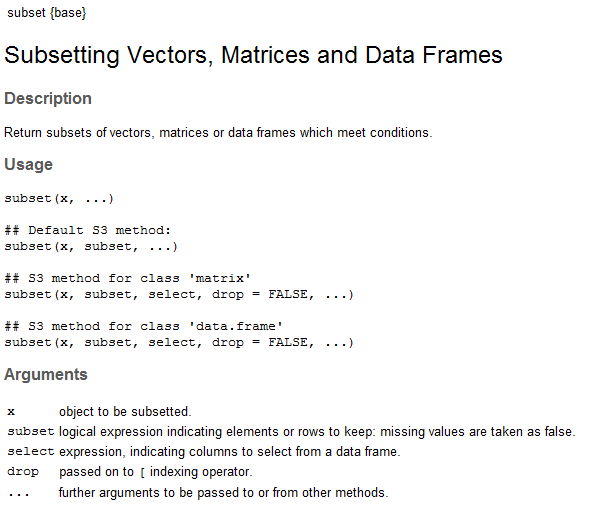
\includegraphics[width=.75\textwidth, height=6cm]{../figure/FunctionSubset.PNG}\\
}
\end{frame}
%%%%%%%%%%%%%%%%%%%%%%%%%%%%%%%%%%%%%%%%%%%%%%%%%%%%%%%%
\begin{frame}[fragile]{Subsetting}
%\frametitle{\vspace{-.05cm}\begin{center}\footnotesize{Subsetting}\end{center}}
\footnotesize{
\begin{Schunk}
\begin{Sinput}
 sub3 <- subset(bm,Commune %in% c("Brecht", "Grimbergen","As","Dinant"))
 sub3$Commune == sub2$Commune
\end{Sinput}
\begin{Soutput}
[1] TRUE TRUE TRUE TRUE
\end{Soutput}
\end{Schunk}


\begin{Schunk}
\begin{Sinput}
 sub4 <- subset(bm,substr(as.character(Commune),1,1)=="B")
 head(sub4[,1:7])
\end{Sinput}
\begin{Soutput}
      Commune   INS Province Arrondiss Men04 Women04 Tot04
3    Boechout 11004        1        11  6027    5927 11954
4        Boom 11005        1        11  7640    8066 15706
5    Borsbeek 11007        1        11  4948    5328 10276
6  Brasschaat 11008        1        11 18142   18916 37058
7      Brecht 11009        1        11 12975   12976 25951
31    Berlaar 12002        1        12  5145    5206 10351
\end{Soutput}
\end{Schunk}
}
\end{frame}
%%%%%%%%%%%%%%%%%%%%%%%%%%%%%%%%%%%%%%%%%%%%%%%%%%%%%%%%
\begin{frame}[fragile]{Loops}
%\frametitle{\vspace{-.05cm}\begin{center}\footnotesize{Loops}\end{center}}

\begin{itemize}
\footnotesize{
\item Loops are convenient when conducting one task several times
\pause\item Very useful for e.g. simulations
\pause\item But: CPU-intensive
\pause\item[$\Rightarrow$] avoid loops if possible (esp. for large datasets)}
\end{itemize}
\pause\footnotesize{
\begin{Schunk}
\begin{Sinput}
 A1 <- vector()
 for(i in 1:10){
+   A1[i] <- sample(1:10,1)
+ }
 A1
\end{Sinput}
\begin{Soutput}
 [1] 10 10  3  9  7  6  8  2  7  8
\end{Soutput}
\end{Schunk}
}
\end{frame}
%%%%%%%%%%%%%%%%%%%%%%%%%%%%%%%%%%%%%%%%%%%%%%%%%%%%%%%%
\begin{frame}[fragile]{Loops}
%\frametitle{\vspace{-.05cm}\begin{center}\footnotesize{Loops}\end{center}}

\begin{itemize}
\footnotesize{
\item To save the results, it is useful to create a container prior to the loop 
}
\end{itemize}
\footnotesize{
\begin{Schunk}
\begin{Sinput}
 A2 <- matrix(nrow = 5,ncol = 2)
 for(i in 1:nrow(A2)){
+   A <- sample(1:50,30)
+   A2[i,1] <- mean(A)
+   A2[i,2] <- var(A)
+ }
 A2
\end{Sinput}
\begin{Soutput}
      [,1]  [,2]
[1,] 27.40 230.7
[2,] 27.50 195.6
[3,] 25.33 221.7
[4,] 29.67 198.0
[5,] 28.40 251.1
\end{Soutput}
\end{Schunk}
}
\end{frame}
%%%%%%%%%%%%%%%%%%%%%%%%%%%%%%%%%%%%%%%%%%%%%%%%%%%%%%%%
\begin{frame}[fragile]{Loops}{Simulation}
%\frametitle{\vspace{-.05cm}\begin{center}\footnotesize{Loops\\ Simulation}\end{center}}
\footnotesize{
\begin{Schunk}
\begin{Sinput}
 data(belgianmunicipalities)
 pik <- inclusionprobabilities(belgianmunicipalities$Tot04,200)
 # Computes the inclusion probabilities
 N <- length(pik)
 # population size
 n <- sum(pik)
 # sample size
 sim <- 1000
 ss <- array(0, c(sim, 5))
 # sim2 <- 10000   #second simulation
 # ss2 <- array(0, c(sim2, 5))
 # number of simulations
 y <- belgianmunicipalities$TaxableIncome
 # variable of interest
 ht <- numeric(5)
 # Horvitz-Thompson estimator for the simulation
\end{Sinput}
\end{Schunk}
}
\end{frame}

%%%%%%%%%%%%%%%%%%%%%%%%%%%%%%%%%%%%%%%%%%%%%%%%%%%%%%%%
\begin{frame}[fragile]{Loops} {Simulation}
%\frametitle{\vspace{-.05cm}\begin{center}\footnotesize{Loops\\ Simulation}\end{center}}
\footnotesize{
\begin{Schunk}
\begin{Sinput}
 for (i in 1:sim) {
+     cat("Step ", i, "\n")
+     s <- UPpoisson(pik)
+     ht[1] <- HTestimator(y[s == 1], pik[s == 1])
+     s <- UPrandomsystematic(pik)
+     ht[2] <- HTestimator(y[s == 1], pik[s == 1])
+     s <- UPsystematic(pik)
+     ht[3] <- HTestimator(y[s == 1], pik[s == 1])
+     s <- sample(y, n,replace = T)
+     ht[4] <- HTestimator(s, rep(n/N,n))
+     s <- srswor(n, N)
+     ht[5] <- HTestimator(y[s == 1], rep(n/N, n))
+     ss[i, ] <- ss[i, ] + ht 
+   } 
\end{Sinput}
\end{Schunk}
}
\begin{itemize}\footnotesize{
\item \R{cat()} can be used to display the simulation step that is recently proceeded
}
\end{itemize}
\tiny{Example based on: Tille,Y and Matai, A. (2010). TEACHING SURVEY SAMPLING WITH THE SAMPLING R PACKAGE. \emph{ICOTS8 (2010) Invited Paper Refereed}}
\end{frame}
%%%%%%%%%%%%%%%%%%%%%%%%%%%%%%%%%%%%%%%%%%%%%%%%%%%%%%%%
\begin{frame}[fragile]{Loops} {Simulation}
%\frametitle{\vspace{-.05cm}\begin{center}\footnotesize{Loops\\ Simulation}\end{center}}
\footnotesize{
\begin{Schunk}
\begin{Sinput}
 # boxplots of the estimators
   par(mfrow=c(1,2))
   boxplot(data.frame(ss), las = 3) 
   boxplot(data.frame(ss2), las = 3)
\end{Sinput}
\end{Schunk}
}
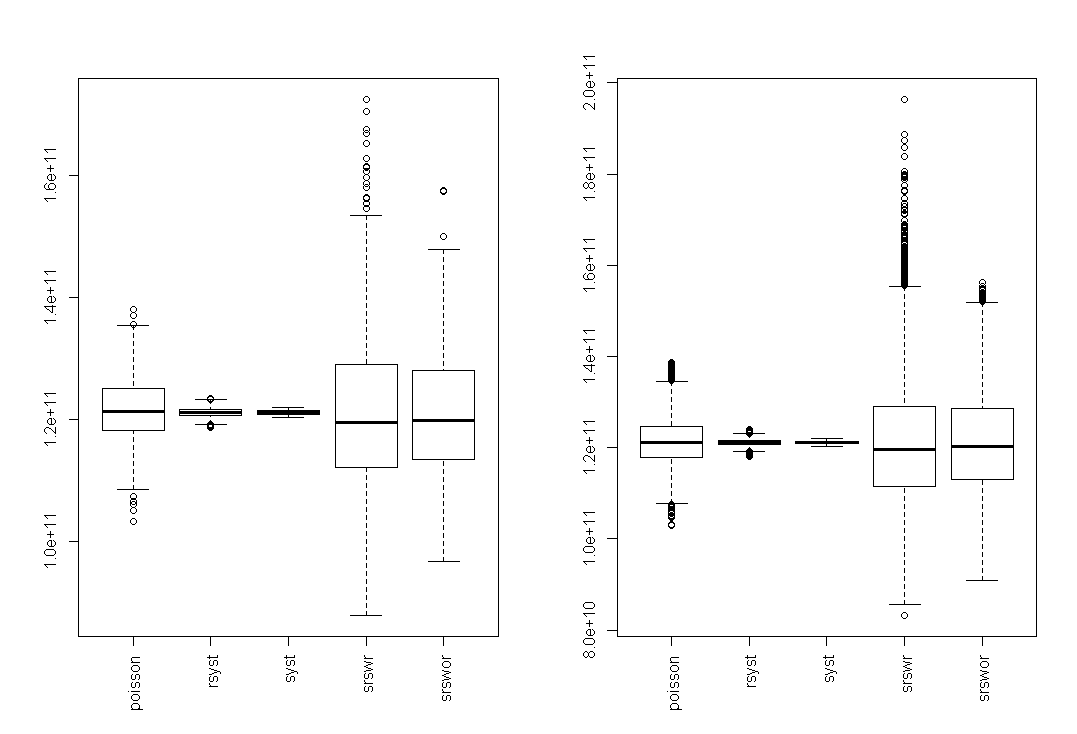
\includegraphics[width=\textwidth, height=6cm]{../figure/Verteilungen.png}

\end{frame}

%%%%%%%%%%%%%%%%%%%%%%%%%%%%%%%%%%%%%%%%%%%%%%%%%%%%%%%%
\begin{frame}[fragile]{The apply function}
%\frametitle{\vspace{-.05cm}\begin{center}\footnotesize{The apply function}\end{center}}
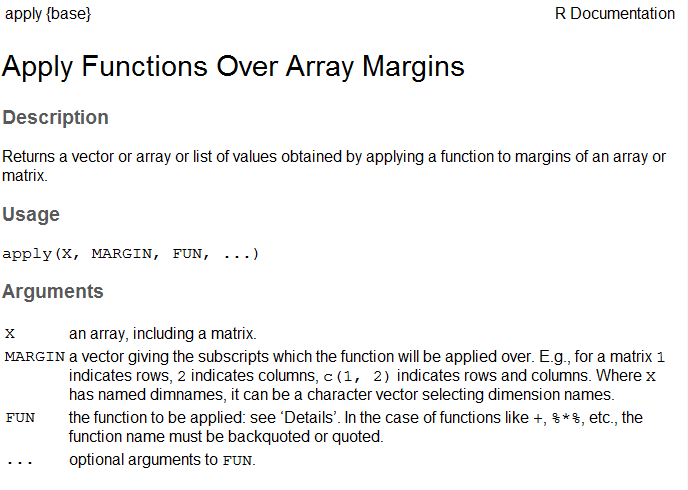
\includegraphics[width=\textwidth, height=6cm]{H:/Sand_Summerschool/SamplingAndEsimation/excercise/figure/FunctionApply.PNG}
\end{frame}
%%%%%%%%%%%%%%%%%%%%%%%%%%%%%%%%%%%%%%%%%%%%%%%%%%%%%%%%
\begin{frame}[fragile]{The apply function}
%\frametitle{\vspace{-.05cm}\begin{center}\footnotesize{The apply function}\end{center}}
\footnotesize{
\begin{itemize}\footnotesize{
\item If \R{margin=1}, the function will be applied to the rows of an array
\item If \R{margin=2}, the function will be applied to the columns of an array
}
\end{itemize}
\vspace{.5cm}
\pause
\begin{Schunk}
\begin{Sinput}
 Applydat <- matrix(1:25, nrow = 5, ncol = 5, byrow = F)
 apply(Applydat,1,mean)
\end{Sinput}
\begin{Soutput}
[1] 11 12 13 14 15
\end{Soutput}
\begin{Sinput}
 apply(Applydat,2,mean)
\end{Sinput}
\begin{Soutput}
[1]  3  8 13 18 23
\end{Soutput}
\end{Schunk}
}
\end{frame}
%%%%%%%%%%%%%%%%%%%%%%%%%%%%%%%%%%%%%%%%%%%%%%%%%%%%%%%%
\begin{frame}[fragile]{The tapply function}
%\frametitle{\vspace{-.05cm}\begin{center}\footnotesize{The tapply function}\end{center}}
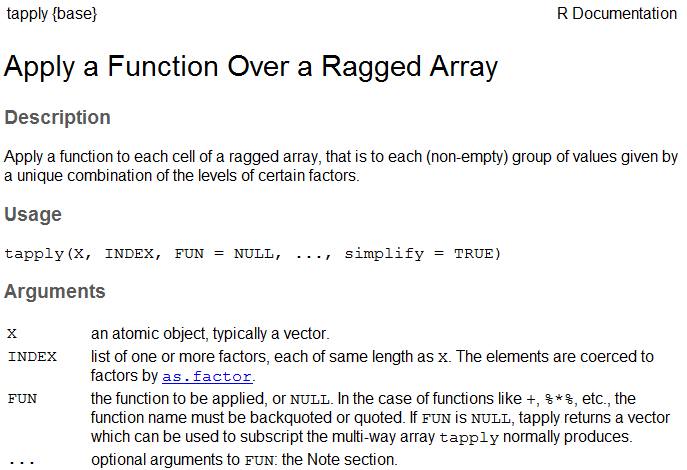
\includegraphics[width=\textwidth, height=6cm]{../figure/FunctionTapply.PNG}
\end{frame}
%%%%%%%%%%%%%%%%%%%%%%%%%%%%%%%%%%%%%%%%%%%%%%%%%%%%%%%%
\begin{frame}[fragile]{The apply function}
%\frametitle{\vspace{-.05cm}\begin{center}\footnotesize{The apply function}\end{center}}
\footnotesize{
\begin{Schunk}
\begin{Sinput}
 Tapplydat <- data.frame(Income = rnorm(6,1400,200),
+                    Gender = sample(c("Male","Female"),6,replace = T))
 Tapplydat
\end{Sinput}
\begin{Soutput}
  Income Gender
1   1703   Male
2   1452   Male
3   1418   Male
4   1376   Male
5   1161 Female
6   1522 Female
\end{Soutput}
\begin{Sinput}
 tapply(Tapplydat$Income, Tapplydat$Gender, mean)
\end{Sinput}
\begin{Soutput}
Female   Male 
  1342   1487 
\end{Soutput}
\end{Schunk}
}
\end{frame}
%%%%%%%%%%%%%%%%%%%%%%%%%%%%%%%%%%%%%%%%%%%%%%%%%%%%%%%%
\begin{frame}[fragile]{Writing your own function}
%\frametitle{\vspace{-.05cm}\begin{center}\footnotesize{Writing your own function}\end{center}}
\begin{center}
\textbf{The finite population correction...}
\end{center}
\vspace{.25cm}
\begin{equation*}
1-f=\frac{N-n}{N}=1-\frac{n}{N}
\end{equation*}\\
\vspace{.5cm}
...can also be turned into a \R{R} function
\begin{Schunk}
\begin{Sinput}
 fpc <- function(N,n){(N-n)/N}
 fpc(100,8)
\end{Sinput}
\begin{Soutput}
[1] 0.92
\end{Soutput}
\end{Schunk}
\end{frame}
%%%%%%%%%%%%%%%%%%%%%%%%%%%%%%%%%%%%%%%%%%%%%%%%%%%%%%%%
\begin{frame}[fragile]{Writing "advanced" functions}
%\frametitle{\vspace{-.05cm}\begin{center}\footnotesize{Writing "advanced" functions}\end{center}}
\footnotesize{
\vspace{-.25cm}
\begin{center}
\textbf{Generating a telephone sample with the approach of Gabler and H\"ader:}
\end{center}
\vspace{.25cm}
Constructing a synthetic frame:
\begin{Schunk}
\begin{Sinput}
 fra <-data.frame(pre = sample(c(30,40,89,221,621),10000,replace = T),
+                  bank = sample(100:99999,10000,replace = T))
 fra[1:4,]
\end{Sinput}
\begin{Soutput}
  pre  bank
1 221  5728
2 221 32661
3 621 64698
4 621 35754
\end{Soutput}
\begin{Sinput}
 fra <- fra[order(fra[,1]),]
 fra[1:4,]
\end{Sinput}
\begin{Soutput}
   pre  bank
11  30 87896
13  30  7164
15  30 63673
16  30 17772
\end{Soutput}
\end{Schunk}
}
\end{frame}
%%%%%%%%%%%%%%%%%%%%%%%%%%%%%%%%%%%%%%%%%%%%%%%%%%%%%%%%
\begin{frame}[fragile]{Writing "advanced" functions}
%\frametitle{\vspace{-.05cm}\begin{center}\footnotesize{Writing "advanced" functions}\end{center}}
\footnotesize{
\begin{Schunk}
\begin{Sinput}
 tel.samp <- function(fra,n){
+   len <- nrow(fra)*100
+   s <- sort(sample(len,n))
+   row <- ceiling(s/100)
+   app <- s%%100
+   ts <- fra[row,]
+   num <- data.frame(prefix = paste("0",ts[,1],sep = ""),
+                     number = paste(ts[,2],app,sep = ""))
+   return(num)
+ }
\end{Sinput}
\end{Schunk}
}

\begin{itemize}\footnotesize{
\item \R{fra} is the sampling frame
\item \R{n} is the sample size
\item with \R{return()}, one can determine the results that the function should display
}
\end{itemize}

\end{frame}
%%%%%%%%%%%%%%%%%%%%%%%%%%%%%%%%%%%%%%%%%%%%%%%%%%%%%%%%
\begin{frame}[fragile]{Writing "advanced" functions}
%\frametitle{\vspace{-.05cm}\begin{center}\footnotesize{Writing "advanced" functions}\end{center}}
\footnotesize{
\begin{Schunk}
\begin{Sinput}
 my.first.ts <- tel.samp(fra,10)
 head(my.first.ts)
\end{Sinput}
\begin{Soutput}
  prefix  number
1    030 4965129
2    030 2690436
3    040 8495419
4    040 7116060
5    040 3043965
6    089 3369754
\end{Soutput}
\end{Schunk}
}

\vspace{.25cm}
\begin{itemize}
\item \R{sort()} sorts an atomic vector in an ascending or descending order and returns the values
\item \R{order()} sorts an atomic vector or a data frame in an ascending or descinding order and returns the row number
\end{itemize}
\end{frame}
%%%%%%%%%%%%%%%%%%%%%%%%%%%%%%%%%%%%%%%%%%%%%%%%%%%%%%%%
\begin{frame}[fragile]{Stratified Random Sampling}
%\frametitle{\vspace{-.05cm}\begin{center}\footnotesize{Stratified Random Sampling}\end{center}}
\footnotesize{
\begin{center}
\textbf{Using a loop to draw stratified random samples}
\end{center}
\begin{Schunk}
\begin{Sinput}
 str.bm <- split(bm,bm$Province)
 nh <- c(2,3,7,3,2,6,7,2,9)
 res <- list()
 for(i in 1:length(str.bm)){
+   ID <- str.bm[[i]]$INS
+   res[[i]] <- sample(ID,nh[i],replace=F)
+ }
 s <- unlist(res)
 result<-bm[bm$INS %in% s,]
 table(result$Province)
\end{Sinput}
\begin{Soutput}
1 2 3 4 5 6 7 8 9 
2 3 7 3 2 6 7 2 9 
\end{Soutput}
\end{Schunk}
}
\end{frame}
%%%%%%%%%%%%%%%%%%%%%%%%%%%%%%%%%%%%%%%%%%%%%%%%%%%%%%%%
\begin{frame}[fragile]{Stratified Random Sampling}
%\frametitle{\vspace{-.05cm}\begin{center}\footnotesize{Stratified Random Sampling}\end{center}}
\footnotesize{
You can also use the \R{strata()} command from the \R{sampling} package
\begin{itemize}
\item[$\Rightarrow$] the function returns the unit's identifier, stratum and its inclusion probability
\end{itemize}
\begin{Schunk}
\begin{Sinput}
 s <- strata(bm,"Province",nh,method = "srswor")
 result1 <- getdata(bm,s)
 head(result1[,c(1:3,ncol(result)-1,ncol(result))])
\end{Sinput}
\begin{Soutput}
                Commune   INS Arrondiss medianincome Province
48               Dessel 13006        13        20212        1
51            Herentals 13011        13        19141        1
89  Woluwe-Saint-Pierre 21019        21        22051        2
151              Linter 24133        24        21053        2
161        Grez-Doiceau 25037        25        21029        2
182             Beernem 31003        31        20268        3
\end{Soutput}
\end{Schunk}
\begin{itemize}
\item[$\Rightarrow$] \R{getdata()} merges the sample-IDs with your original dataset and returns your sample as a data frame
\end{itemize}
}
\end{frame}
%%%%%%%%%%%%%%%%%%%%%%%%%%%%%%%%%%%%%%%%%%%%%%%%%%%%%%%%
\begin{frame}[fragile]{Stratified Random Sampling}
%\frametitle{\vspace{-.05cm}\begin{center}\footnotesize{Stratified Random Sampling}\end{center}}
\vspace{-.35cm}
\footnotesize{
\begin{center}
\textbf{Proportional Allocation:}
\end{center}
\begin{equation*}
\gamma_{h}=\frac{N_h}{N}
\end{equation*}

\begin{equation*}
n_h=n*\gamma_{h}
\end{equation*}

\begin{Schunk}
\begin{Sinput}
 n <- 30
 gamma <- prop.table(table(bm$Province))
 nh <- n*gamma
 t(nh)
\end{Sinput}
\begin{Soutput}
           1     2     3     4     5     6     7     8     9
  [1,] 3.565 5.654 3.260 3.311 3.514 4.278 2.241 2.241 1.935
\end{Soutput}
\begin{Sinput}
 s <- strata(bm,"Province",nh,"srswor")
 result.p <- getdata(bm,s)
 nrow(result.p)
\end{Sinput}
\begin{Soutput}
[1] 26
\end{Soutput}
\end{Schunk}
\begin{itemize}
\item[$\Rightarrow$] the \R{strata()} command generally rounds down
\item[$\Rightarrow$] use \R{round()} or the cox-algorithm
\end{itemize}
}
\end{frame}
%%%%%%%%%%%%%%%%%%%%%%%%%%%%%%%%%%%%%%%%%%%%%%%%%%%%%%%%
\begin{frame}[fragile]{Stratified Random Sampling}
%\frametitle{\vspace{-.05cm}\begin{center}\footnotesize{Stratified Random Sampling}\end{center}}
\vspace{-.35cm}
\footnotesize{
\begin{center}
\textbf{Optimal Allocation:}
\end{center}
\begin{equation*}
n_h=n*\frac{\gamma_{h}\sigma_{h}}{\sum_{g=1}^{L}\gamma_{g}\sigma_{g}}=n*\frac{N_{h}\sigma_{h}}{\sum_{g=1}^{L}N_{g}\sigma_{g}} \text{         ~~~~~~ } h=1,\ldots,L
\end{equation*}

\vspace{.25cm}
\pause\textbf{Step 1:} getting $Var(\overline{y}_{StrRS,opt})$
\begin{equation*}
Var(\overline{y}_{StrRS,opt})=\frac{1}{n}\sum_{h=1}^{L}(\gamma_h*\sigma_h)^2=\frac{1}{n}\sum_{h=1}^{L}(\frac{N_h}{N}\sigma_h)^2=\frac{1}{N^2}\sum_{h=1}^{L}\frac{N_h^2}{n_h}\sigma_h^2
\end{equation*}
\begin{Schunk}
\begin{Sinput}
 GetStratVar <- function(Y, sind, nh) {
+   Nh <- tapply(sind,sind,length)
+   N <- length(sind)
+   sum(Nh^2*tapply(Y,sind,function(x) 
+     var(x)*(length(x)-1)/length(x))/nh)/N^2
+ }
 GetStratVar(bm$Tot04,bm$Province,rep(5,length(unique(bm$Province))))
\end{Sinput}
\begin{Soutput}
[1] 18941644
\end{Soutput}
\end{Schunk}
}
\end{frame}
%%%%%%%%%%%%%%%%%%%%%%%%%%%%%%%%%%%%%%%%%%%%%%%%%%%%%%%%
\begin{frame}[fragile]{Stratified Random Sampling}
%\frametitle{\vspace{-.05cm}\begin{center}\footnotesize{Stratified Random Sampling}\end{center}}
\vspace{-.35cm}
\footnotesize{
\textbf{Step 2:} calculating $n_h$
\begin{Schunk}
\begin{Sinput}
 GetOptAlloc <- function(Y, sind, n){
+   L <- length(unique(sind))
+   nh <- rep(2,L)
+   Nh <- tapply(sind,sind,length)
+   v <- numeric(L)
+   M <- diag(rep(1,L))
+   while (sum(nh) < n) {
+     for (i in 1:L) {
+       if (nh[i] == Nh[i]) {
+         v[i] <- Inf
+       } else {
+         v[i] <- GetStratVar(Y, sind, nh + M[,i])
+       }
+     }
+     nh <- nh + M[,which.min(v)]
+   }
+   nh
+ } 
\end{Sinput}
\end{Schunk}

}
\end{frame}
%%%%%%%%%%%%%%%%%%%%%%%%%%%%%%%%%%%%%%%%%%%%%%%%%%%%%%%%
\begin{frame}[fragile]{Stratified Random Sampling}
%\frametitle{\vspace{-.05cm}\begin{center}\footnotesize{Stratified Random Sampling}\end{center}}
\vspace{-.35cm}
\footnotesize{
\begin{Schunk}
\begin{Sinput}
 nh <- GetOptAlloc(bm$Tot04,bm$Province,50)
 t(nh)
\end{Sinput}
\begin{Soutput}
     [,1] [,2] [,3] [,4] [,5] [,6] [,7] [,8] [,9]
[1,]   13    9    4    6    6    6    2    2    2
\end{Soutput}
\begin{Sinput}
 nh2 <- GetOptAlloc(bm$averageincome,bm$Province,50)
 t(nh2)
\end{Sinput}
\begin{Soutput}
     [,1] [,2] [,3] [,4] [,5] [,6] [,7] [,8] [,9]
[1,]    6   14    4    5    6    6    2    4    3
\end{Soutput}
\end{Schunk}
\begin{itemize}
\pause\item[$\Rightarrow$] Allocation differs depending on the variable of interest
\end{itemize}
}
\end{frame}
%%%%%%%%%%%%%%%%%%%%%%%%%%%%%%%%%%%%%%%%%%%%%%%%%%%%%%%%
\begin{frame}[fragile]{Cluster Sampling}
%\frametitle{\vspace{-.05cm}\begin{center}\footnotesize{Cluster Sampling}\end{center}}
\vspace{-.35cm}
\footnotesize{
\begin{center}
\textbf{Simple Method:}
\end{center}
\begin{itemize}
\item[$\Rightarrow$] Sample cluster proportional to size; sample all units within a cluster
\end{itemize}
\begin{Schunk}
\begin{Sinput}
 l <- 4
 gamma <- prop.table(table(bm$Province))
 clus <- sample(unique(bm$Province),l, prob = gamma, replace = F)
 res.clus <- bm[bm$Province %in% clus,]
 nrow(res.clus)
\end{Sinput}
\begin{Soutput}
[1] 303
\end{Soutput}
\end{Schunk}

\begin{itemize}
\pause\item[$\Rightarrow$] Sample size varies
\end{itemize}
}
\end{frame}
%%%%%%%%%%%%%%%%%%%%%%%%%%%%%%%%%%%%%%%%%%%%%%%%%%%%%%%%
\begin{frame}[fragile]{Cluster Sampling}
%\frametitle{\vspace{-.05cm}\begin{center}\footnotesize{Cluster Sampling}\end{center}}
\vspace{-.35cm}
\footnotesize{
\begin{center}
\textbf{Fixed Sample Size:}
\end{center}
\begin{itemize}
\item[$\Rightarrow$] Sample cluster proportional to size; sample the same number of units within each cluster
\end{itemize}
\begin{Schunk}
\begin{Sinput}
 l <- 4
 gamma <- prop.table(table(bm$Province))
 clus <- sample(unique(bm$Province),l, prob = gamma, replace = F)
 fixed.res.clus <-list()
 for(i in 1:l){
+   nh <- 30
+   bm.cl <- bm[bm$Province == clus[i],]
+   fixed.res.clus[[i]] <- sample(bm.cl$INS,nh, replace = F)
+ }
 ID <- unlist(fixed.res.clus)
 fixed.clus <- bm[bm$INS %in% ID,]
 nrow(fixed.clus)
\end{Sinput}
\begin{Soutput}
[1] 120
\end{Soutput}
\end{Schunk}
}
\end{frame}
%%%%%%%%%%%%%%%%%%%%%%%%%%%%%%%%%%%%%%%%%%%%%%%%%%%%%%%%
\begin{frame}[fragile]{Cluster Sampling}
%\frametitle{\vspace{-.05cm}\begin{center}\footnotesize{Cluster Sampling}\end{center}}
\footnotesize{
The \R{sample} package also offers a cluster function
\begin{Schunk}
\begin{Sinput}
 l <- 4
 sam.clus <- cluster(bm,"Province",4,method = "srswor")
 res.clus.samp <- getdata(bm,sam.clus)
 nrow(res.clus.samp)
\end{Sinput}
\begin{Soutput}
[1] 216
\end{Soutput}
\end{Schunk}
\begin{itemize}
\item[$\Rightarrow$] Samples all units within a cluster
\end{itemize}
}
\end{frame}
%%%%%%%%%%%%%%%%%%%%%%%%%%%%%%%%%%%%%%%%%%%%%%%%%%%%%%%%
\begin{frame}[fragile]{Mean and Variance} {of different Sampling Designs}
%\frametitle{\vspace{-.05cm}\begin{center}\footnotesize{Mean and Variance\\ of different sampling designs}\end{center}}
\vspace{-.5cm}
\footnotesize{
\begin{center}
\textbf{Mean: Simple Random Sampling (SRS)}
\end{center}
\begin{equation*}
\overline{y}_{SRS}=\frac{1}{n}\sum_{i=1}^{n}y_i
\end{equation*}
}
\begin{Schunk}
\begin{Sinput}
 SRS.mean <- function(Y,S){return(mean(Y[S]))}
\end{Sinput}
\end{Schunk}
\footnotesize{
\begin{center}
\textbf{Variance: Simple Random Sampling (SRS)}
\end{center}
\begin{equation*}
V(\overline{y}_{SRS})=\frac{\sigma^2}{n}\text{; ~~~~ } V(\overline{y}_{SRSWOR})=\frac{N-n}{N-1}\frac{\sigma^2}{n}=(1-\frac{n}{N})\frac{S^2}{n}
\end{equation*}
\begin{equation*}
\hat{V}(\overline{y}_{SRSWOR})=(1-\frac{n}{N})\frac{s^2}{n}
\end{equation*}
\begin{Schunk}
\begin{Sinput}
 SRS.evar <- function(Y,S){return(var(Y[S])/length(S))}
 SRSWOR.evar <- function(Y,S)
+   {return(fpc(nrow(Y),length(S))*var(Y[S])/length(S))}
\end{Sinput}
\end{Schunk}
}
\end{frame}
%%%%%%%%%%%%%%%%%%%%%%%%%%%%%%%%%%%%%%%%%%%%%%%%%%%%%%%%
\begin{frame}[fragile]{Mean and Variance} {of different Sampling Designs}
%\frametitle{\vspace{-.05cm}\begin{center}\footnotesize{Mean and Variance\\ of different sampling designs}\end{center}}
\vspace{-.5cm}
\footnotesize{
\begin{center}
\textbf{Mean: Stratified Random Sampling (StrRS)}
\end{center}
\begin{equation*}
\hat{\overline{y}}_{StrRS}=\sum_{h=1}^{L}\gamma_{h}\frac{1}{n_h}\sum_{i=1}^{n_h}y_i
\end{equation*}
\vspace{.25cm}
\begin{Schunk}
\begin{Sinput}
 Strat.mean <- function(Y,sind,S){
+   Nh <- tapply(Y,sind,length)
+   Str.mean <- sum(Nh*tapply(Y[S], sind[S], mean) / sum(Nh))
+   return(Str.mean)
+ }
 S <- as.numeric(row.names(result))
 Strat.mean(bm$averageincome,bm$Province,S)
\end{Sinput}
\begin{Soutput}
[1] 24000
\end{Soutput}
\end{Schunk}
\begin{itemize}
\item \R{Y} is the variable of interest
\item \R{sind} is the identifier of the strata (\R{length(Y)})
\item \R{S} are the row names of the sample 
\end{itemize}

}
\end{frame}
%%%%%%%%%%%%%%%%%%%%%%%%%%%%%%%%%%%%%%%%%%%%%%%%%%%%%%%%
\begin{frame}[fragile]{Mean and Variance} {of different Sampling Designs}
%\frametitle{\vspace{-.05cm}\begin{center}\footnotesize{Mean and Variance\\ of different sampling designs}\end{center}}
\footnotesize{
\vspace{-.5cm}
\begin{center}
\textbf{Variance: Stratified Random Sampling (StrRS)}
\end{center}
\begin{equation*}
V(\overline{y}_{StrRS})=\sum_{h=1}^{L}\gamma_{h}^2\frac{\sigma_h^2}{n_h}\text{;~~~~~~~~~~~~}V(\overline{y}_{StrRSWOR})=\sum_{h=1}^{L}\gamma_{h}^2\frac{\sigma_h^2}{n_h}*\frac{N_h-n_h}{N_h-1}
\end{equation*}
\begin{equation*}
\hat{V}(\overline{y}_{StrRS})=\sum_{h=1}^{L}\gamma_{h}^2\frac{s_h^2}{n_h}\text{;~~~~~~~~~~~~}\hat{V}(\overline{y}_{StrRSWOR})=\sum_{h=1}^{L}\gamma_{h}^2\frac{s_h^2}{n_h}*\frac{N_h-n_h}{N_h}
\end{equation*}
\vspace{.25cm}
\begin{Schunk}
\begin{Sinput}
 Strat.evar<- function(Y, sind, S) {
+   Nh <- tapply(sind,sind,length)
+   nh <- tapply(sind[S], sind[S], length)
+   ssh <- tapply(Y[S], sind[S], var)
+   res <- sum((Nh/sum(Nh))^2*ssh/nh*(Nh-nh)/Nh)
+   return(res)
+ }
 S <- as.numeric(row.names(result))
 Strat.evar(bm$averageincome,bm$Province,S)
\end{Sinput}
\begin{Soutput}
[1] 256082
\end{Soutput}
\end{Schunk}
}
\end{frame}
%%%%%%%%%%%%%%%%%%%%%%%%%%%%%%%%%%%%%%%%%%%%%%%%%%%%%%%%
\begin{frame}[fragile]{Mean and Variance} {of different Sampling Designs}
%\frametitle{\vspace{-.05cm}\begin{center}\footnotesize{Mean and Variance\\ of different sampling designs}\end{center}}
\vspace{-.5cm}
\footnotesize{
\begin{center}
\textbf{Mean: One-Stage Cluster Sampling (SRCS)}
\end{center}
\begin{equation*}
\hat{\overline{y}}_{SRCS}=\frac{L}{l}\sum_{h=1}^{l}\gamma_{h}^a*\overline{y}_h^a=\frac{L}{l}\sum_{h=1}^{l}*\frac{N_h^a}{\sum_{g=1}^{L}N_g^a}*\frac{1}{N_h^a}\sum_{i=1}^{N_h^a}Y_{ih}
\end{equation*}
\vspace{.25cm}
\begin{Schunk}
\begin{Sinput}
 SRCS.mean <-function(Y,sind,S){
+   L <- length(unique(sind))
+   l <- length(unique(sind[S]))
+   N <- length(Y)
+   N_h_a <- tapply(Y[S],sind[S],length)
+   mu_h_a <- tapply(Y[S],sind[S],mean)
+   return(L/l*sum(N_h_a/N*mu_h_a))
+ }
 Sc <- as.numeric(row.names(res.clus))
 SRCS.mean(bm$averageincome,bm$Province,Sc)
\end{Sinput}
\begin{Soutput}
[1] 30483
\end{Soutput}
\end{Schunk}
}
\end{frame}
%%%%%%%%%%%%%%%%%%%%%%%%%%%%%%%%%%%%%%%%%%%%%%%%%%%%%%%%
\begin{frame}[fragile]{Mean and Variance} {of different Sampling Designs}
%\frametitle{\vspace{-.05cm}\begin{center}\footnotesize{Mean and Variance\\ of different sampling designs}\end{center}}
\vspace{-.5cm}
\footnotesize{
\begin{center}
\textbf{Mean: One-Stage Cluster Sampling (SRCS)}
\end{center}
\begin{equation*}
V(\overline{y}_{SRCS})=\frac{L^2}{N^2}*\frac{\sigma_e^2}{l}*\frac{L-l}{L-1}
\end{equation*}
\begin{equation*}
\hat{V}(\overline{y}_{SRCS})=\frac{L^2}{N^2}*\frac{s_e^2}{l}*\frac{L-l}{L}\text{;}
\end{equation*}
\begin{equation*}
s_e^2=\frac{1}{l-1}\sum_{r=1}^{l}(N_r^{a}\overline{y}_r^{a}-\frac{N*\hat{\overline{y}}_{SRCS}}{L})^2
\end{equation*}
Calculating $s_e^2$
\begin{Schunk}
\begin{Sinput}
 se.sq <- function(Y,sind,S){
+   L <- length(unique(sind))
+   l <- length(unique(sind[S]))
+   N <- length(Y)
+   mu.SRCS <- SRCS.mean(Y,sind,S)
+   c <- N*mu.SRCS/L
+   mu_h_a <- tapply(Y[S],sind[S],mean)
+   N_h_a <- tapply(Y[S],sind[S],length)
+  return ( 1/(l-1)*sum((N_h_a*mu_h_a-c)^2))
+ }
\end{Sinput}
\end{Schunk}
}
\end{frame}
%%%%%%%%%%%%%%%%%%%%%%%%%%%%%%%%%%%%%%%%%%%%%%%%%%%%%%%%
\begin{frame}[fragile]{Mean and Variance} {of different Sampling Designs}
%\frametitle{\vspace{-.05cm}\begin{center}\footnotesize{Mean and Variance\\ of different sampling designs}\end{center}}
\vspace{-.5cm}
\footnotesize{
Calculating $\hat{V}(\overline{y}_{SRCS})$
\begin{Schunk}
\begin{Sinput}
 SRCS.evar <- function(Y,sind,S){
+   L <- length(unique(sind))
+   l <- length(unique(sind[S]))
+   N <- length(Y)
+   part1 <- L^2/N^2
+   part2 <- se.sq(Y,sind,S)/l
+   part3 <- (L-l)/L
+   return(part1*part2*part3)
+ }
 Sc <- as.numeric(row.names(res.clus))
 SRCS.evar(bm$averageincome,bm$Province,Sc)
\end{Sinput}
\begin{Soutput}
[1] 28973878
\end{Soutput}
\end{Schunk}
}
\end{frame}
%%%%%%%%%%%%%%%%%%%%%%%%%%%%%%%%%%%%%%%%%%%%%%%%%%%%%%%%%%%%%%%%%%%%%%%%%%%
\begin{frame}[fragile]{Exercise 3}
%\frametitle{\vspace{-.05cm}\begin{center}\footnotesize{Exercise 3}\end{center}}
\vspace{-.25cm}
\begin{exampleblock}{Sampling and Estimation}
\begin{enumerate}\footnotesize{
\item Load the \R{belgianmunicipalities} data and allocate the sample size \alert{$n=180$} to the provinces
\begin{itemize}
\item equal allocation
\item proportional to the number of communes 
\item proportional to the average income 
\item proportional to the taxable income 
\item under optimal allocation for the variable \R{Tot04}
\end{itemize}
\item Furthermore, draw the following two cluster samples
\begin{itemize}
\item two full provinces
\item six full provinces
\end{itemize}
\item Draw \alert{$R=1,000$} samples for each of the allocations and calculate the sample mean of variable \R{Tot04} and its variance for each simulation step
\item Calculate the average mean and variance over the 1,000 simulation steps
\item Calculate the deviation and compare it over the different sampling designs
\item Compare the average variance for each sampling design
}
\end{enumerate}
\end{exampleblock}

\end{frame}
%%%%%%%%%%%%%%%%%%%%%%%%%%%%%%%%%%%%%%%%%%%%%%%%%%%%%%%%%%%%%%%%%%%%%%%%%%%
\begin{frame}[fragile]{Exercise 3}
%\frametitle{\vspace{-.05cm}\begin{center}\footnotesize{Exercise 3}\end{center}}
\footnotesize{
\begin{center}
\textbf{Variance equal allocation}
\end{center}
\begin{equation*}
\hat{V}(\overline{y}_{StrRS,eq})=\frac{1}{n}\sum_{h=1}^{L}\gamma_h^2*s_h^2*\frac{N_h*L-n}{N_h-1}
\end{equation*}
\vspace{.5cm}
\begin{Schunk}
\begin{Sinput}
 Strat.eq.evar <- function(Y,sind,S){
+   L <- length(unique(sind))
+   Nh <- tapply(sind,sind,length)
+   nh <- tapply(sind[S], sind[S], length)
+   ssh <- tapply(Y[S], sind[S], var)
+   res <- 1/sum(nh)*sum((Nh/sum(Nh))^2*
+               ssh*((Nh*L-sum(nh))/(Nh-1)))
+   return(res)
+ }
\end{Sinput}
\end{Schunk}

}
\end{frame}
\begin{frame}[fragile]{Exercise 3}
%\frametitle{\vspace{-.05cm}\begin{center}\footnotesize{Exercise 3}\end{center}}
\footnotesize{
\begin{center}
\textbf{Variance optimal allocation}
\end{center}
\begin{equation*}
\hat{V}(\overline{y}_{StrRS,opt})=\frac{1}{n}(\sum_{h=1}^{L}\gamma_h*s_h)^2-\frac{1}{N}\sum_{h=1}^{L}\gamma_hs_h^2
\end{equation*}
\vspace{.5cm}
\begin{Schunk}
\begin{Sinput}
 Strat.opt.evar <- function(Y, sind, S){
+   Nh <- tapply(sind,sind,length)
+   nh <- tapply(sind[S], sind[S], length)
+   ssh <- tapply(Y[S], sind[S], var)
+   part1 <- 1/sum(nh)*sum(Nh/sum(Nh)*sqrt(ssh))^2
+   part2 <- 1/sum(Nh)*sum(Nh/sum(Nh)*ssh)
+   return(part1-part2)
+ }
\end{Sinput}
\end{Schunk}

}
\end{frame}


\end{document}
